\documentclass[]{report}

\usepackage{amsmath}
\DeclareMathOperator{\Lapl}{\mathcal{L}}
\DeclareMathOperator{\bigO}{\mathcal{O}}

\usepackage[bottom]{footmisc}

\usepackage[backend=bibtex, natbib=true, style=numeric, sorting=none]{biblatex}
\addbibresource{bib.bib}

\usepackage{graphicx}

\usepackage{enumitem}

\title{Spectral Graph Theory and High Performance Computing \\ Master Thesis}
\author{David Wobrock\ \texttt{david.wobrock@gmail.com}}

\begin{document}

\begin{titlepage}
 \maketitle
\end{titlepage}

\tableofcontents
\newpage

\chapter{Introduction}

\section{Background}

\paragraph{}
The talk \cite{siam_slides_2016} and articles \cite{glide_2014} \cite{talebi_nonlocal_2014} by Milanfar, working at Google Research, about using the graph Laplacian operator for nonconformist image processing purposes awakes curiosity.

Indeed, Milanfar reports that these techniques to build image filters are used on smartphones, which implies a reasonable execution time with limited computational resources.
Over 2 billion photos are shared daily on social media \cite{siam_slides_2016}, with very high resolutions and most of the time some processing or filter is applied to them.
The algorithm must be efficient to be deployed at such scale.

\section{Objective}

\paragraph{}
The aim of this degree project is not to explore and improve the state of image processing.
Instead, the spectral methods used in the algorithm will be our focus point.
Those will inevitably expose eigenvalue problems, which may involve solving systems of linear equations.

Concerning the challenges about solving linear systems, on one hand, the size of the systems can be large considering high-resolution images with millions of pixels, or even considering 3D images.
We handle huge matrices of size \(N^2\), with \(N\) the number of pixels of the input image.
On the other hand, images are dense matrices and so will be the matrices we compute, thus also the exposed linear systems.
Often, linear systems result from discretising partial differential equations yielding sparse matrices, and therefore most linear solvers are specialised in sparse systems.

We want to explore the performance of linear solvers on dense problems, their stability and convergence.
This will include preconditioning the linear systems, especially using domain decomposition methods, and analyse their behavior on dense systems.

\section{Related work}

\paragraph{}
In this section, we start by a summary of spectral graph theory as an introduction to the project.
It is followed by image processing techniques for denoising, with traditional patch-based methods and global image filters.
And we finish by a quick overview of linear solvers.

\subsection{Spectral graph theory}

\paragraph{}
Spectral graph theory has a long history starting with matrix theory and linear algebra that were used to analyse adjacency matrices of graphs.
It consists in studying the properties of graphs in relation to the eigenvalues and eigenvectors of the adjacency or Laplacian matrix.
The eigenvalues of such a matrix are called the spectrum of the graph.
The second smallest eigenvalue has been called ``algebraic connectivity of a graph" by Fiedler \cite{fiedler_algebraic_1973}, and is therefore also known as \textit{Fiedler value}, because it contains interesting information about the graph.
Indeed, it can show if the graph is connected, and by extending this property, we can count the number of connected components in the graph through the eigenvalues of the graph Laplacian and do graph partitioning.

The field of spectral graph theory is very broad and the eigendecomposition of graphs is used in a lot of areas.
Spectral graph theory has many applications such as graph colouring, graph isomorphism testing, random walks and graph partitioning among others.

One of the most complete works about spectral graph theory is \cite{chung_spectral_1997} by Fan Chung.
This monograph exposes many properties of graphs, the power of the spectrum and how spectral graph theory links the discrete world to the continuous one.

\paragraph{Laplacian matrix}
Since the adjacency matrix of a graph only holds basic information about it, we usually augment it to the Laplacian matrix.
Multiple definitions of the Laplacian matrix are given in \cite{chung_spectral_1997} and \cite{siam_slides_2016}, and each one has different properties.
The most common ones are the normalised Laplacian and the Random Walk Laplacian.
However, more convenient formulations, like the ``Sinkhorn" Laplacian \cite{milanfar_symmetrizing_2013} and the re-normalised Laplacian \cite{siam_slides_2016} \cite{milanfar_new_2016}, have been proposed since.

\paragraph{The Spectral Theorem}
Some Laplacian definitions result in a symmetric matrix, which is a property that is particularly interesting for spectral theory because of the Spectral Theorem \cite{zhang_spectral_2010}.
Let \(S\) be a real symmetric matrix of dimension \(n\), \(\Phi = [\phi_1 \phi_2 \dots \phi_n ]\) the matrix of eigenvectors of \(S\) and \(\forall i \in [0,n]\), let \(\Pi = diag\{\lambda_i\}\) the diagonal matrix of the eigenvalues of \(S\), then
\[S = \Phi \Pi \Phi^T = \sum_{i=1}^n \lambda_i \phi_i \phi_i^T,\]
the eigendecomposition of \(S\).
We note that the eigenvalues of \(S\) are real and that the eigenvectors are orthogonal, i.e., \(\Phi^T\Phi = I\), with \(I\) the identity matrix.

%\paragraph{Cheeger's inequality}
%One of the most fundamental theorems of spectral graph theory concerns the Cheeger's inequality and Cheeger constant.
%It approximates the sparsest cut of a graph with the second eigenvalue of its Laplacian.
%
%The Cheeger constant \cite{cheeger_lower_1969} measures the degree of ``bottleneck" of a graph, useful for constructing well-connected graphs.
%Considering a graph \(G\) of \(n\) vertices, the Cheeger constant \(h\) is defined as
%\[h(G) = min_{0 < |S| \le \frac{n}{2}} \frac{|\partial S|}{|S|},\]
%where \(S\) is a subset of the vertices of \(G\) and \(\partial S\) is the \textit{edge boundary} of \(S\) to have all edges with exactly one endpoint in \(S\), or formally
%\[\partial S = {{u, v} \in V(G) : u \in S, v \notin S},\]
%with \(V(G)\) the vertices of graph \(G\).
%
%Cheeger's inequality defines a bound and relationship on the smallest positive eigenvalue of the Laplacian matrix \(\Lapl \) such as
%\[\lambda_1(\Lapl) \ge \frac{h^2(\Lapl)}{4}.\]
%
%When the graph \(G\) is \(d\)-regular, thanks to \cite{cvetkovic_spectra_1980}, we also have an inequality between \(h(G)\) and the second smallest eigenvalue \(\lambda_2\) such as
%\[\frac{1}{2}(d-\lambda_2) \le h(G) \le \sqrt{2d(d-\lambda_2)},\]
%where \(d - \lambda_2\) is also called the \textit{spectral gap}.

\paragraph{}
The Laplacian is the foundation of the heat equation, fluid flow and essentially all diffusion equations.
It can generally be thought that the Laplacian operator is a center-surround average \cite{siam_slides_2016} of a given point.
Therefore, applying it on an image results in smoothing.
Generally, applying the graph Laplacian operator on an image provides useful information about it and enables possibilities of interesting image processing techniques.

\subsection{Image processing - denoising}

\paragraph{Background}
Even with high quality cameras, denoising and improving a taken picture remains important.
The two main issues that have to be addressed by denoising are blur and noise.
The effect of blur is internal to cameras since the number of samples of the continuous signal is limited and it should hold the Shannon-Nyquist theorem \cite{buades_review_2005}, stipulating a sufficient condition on the number of samples required to discretise a countinous signal without losing information.
Noise comes from the light acquisition system that fluctuates in relation to the amount of incoming photons.

To model these problems, a classical approach to formulate the deficient image considers \(z\) the clean signal vector, \(e\) a noise vector of variance \(\sigma^2\) and \(y\) the noisy picture:
\[y = z + e.\]

What we want is a high-performance denoiser, capable of scaling up in relation to increasing the image size and keeping reasonable performances.
The output image should come as close as possible to the clean image.
As an important matter, it is now generally accepted that images contain a lot of redundancy.
This means that, in a natural image, every small enough window has many similar windows in the same image.

\paragraph{Traditional, patch-based methods}
The image denoising algorithms review proposed by \cite{buades_review_2005} suggests that the non-local means algorithm, compared to other reviewed methods, comes closest to the original image when applied to a noisy image.
This algorithm takes advantage of the redundancy of natural images and for a given pixel predicts its value by using the pixels in its neighbourhood.

In \cite{dabov_image_2007}, the authors propose the BM3D algorithm, a denoising strategy based on grouping similar 2D blocks of the image into 3D data arrays.
Then, collaborative filtering is performed on these groups and return 2D estimates of all grouped blocks.
This algorithm exposed state-of-the-art performance in terms of denoising at that time.
The results are still one of the best for a reasonable computational cost.

\paragraph{Global filter}
In the last couple of years, global image denoising filters came up, based on spectral decompositions \cite{glide_2014}.
This approach considers the image as a complete graph, where the filter value of each pixel is computed by all pixels in the image.
We define the result image \(z\), \(W\) the huge data-dependent global filter of size \(N \times N\), with \(N\) the number of pixels and the input image \(y\):
\[z = Wy.\]
To show an example of the size of the filter, a standard 10 MPixel picture will result in a filter matrix of \(10^{14}\) elements, taking 800 TB of memory.
This kind of filter is considered in this report.

Those huge matrices will need to be approximated using their eigendecomposition.
And these will need to solve systems of linear equations.

\subsection{Linear solvers and domain decomposition methods}

\paragraph{}
Solving a system of linear equations such that
\[Ax = b,\]
is often critical in scientific computing.
When discretising equations coming from physics for example, a huge linear system can be obtained.
Multiple methods exist to solve such systems, even when the system is large and expensive to compute.
We present in the following the most used and known solvers.

\paragraph{Direct solvers}
The most commonly used solvers for systems of linear equations are direct solvers.
They provide robust methods and optimal solutions to the problem.
However, they can be hard to parallelise and have difficulties with large input.
The most famous is the backslash operator from MATLAB which performs tests to determine which special case algorithm to use, but ultimately falls back on a LU factorisation \cite{mldivide_matlab}.
The LU factorisation, which is a Gaussian elimination, is hard to parallelise.
Although, a block version of the LU factorisation exists that can be parallelised more easily.
There are other parallel direct solvers, like MUMPS \cite{MUMPS_2001}, but generally they reach their computational limit above \(10^6\) degrees of freedom in a 2D problem, and \(10^5\) in 3D.

\paragraph{Iterative solvers}
For larger problems, iterative methods must be used to achieve reasonable runtime performances.
The two types of iterative solvers are fixed-point iteration methods and Krylov type methods.
Both require only a small amount of memory and can often be parallelised.
The main drawback is that these methods tend to be less robust than direct solvers and convergence depends on the problem.
Indeed, ill-conditioned input matrices will be difficult to solve correctly by iterative methods and do not necessarily converge.
Generally, Krylov methods are preferred over fixed-point iteration methods.
The most relevant iterative Krylov methods are the Conjugate Gradient (CG) and the Generalised Minimal Residual method (GMRES) \cite{saad_iterative_2003} \cite{saad_gmres_1986}.

To tackle the ill-conditioned matrices problem, there is a need to precondition the system.


\paragraph{Preconditioners - Domain decomposition methods}
One of the ways to precondition systems of linear equations is to use domain decomposition.
The idea goes back to Schwarz who wanted to solve a Poisson problem on a complex geometry.
He decomposed the geometry into multiple smaller simple geometric forms, making it easy to work on subproblems.
This idea has been extended and improved to propose fixed-point iterations solvers for linear systems.
However, Krylov methods expose better results and faster convergence, but domain decomposition methods can actually be used as preconditioners to the system.
Famous Schwarz preconditioners are the Restricted Additive Schwarz method (RAS) and the Additive Schwarz Method (ASM).
With \(M^{-1}\) the preconditioning matrix, we shall solve
\[M^{-1}Ax = M^{-1}b\]
which exposes the same solution as the original problem.

\paragraph{}
Domain decomposition methods will also be an important topic of this degree project.
These methods are usually applied to solve problems of linear algebra involving partial differential equations (PDEs).
Solving the discretised problem leads to solving linear systems.

Our main reference will be \cite{dolean_domain_2015} which focuses on the parallel linear iterative solvers for systems of linear equations.
Domain decomposition methods are naturally parallel which is convenient for the current state of processor progress.
Without going into the details, we will make use of Schwarz methods for preconditioning and iterative Krylov subspace methods as solvers.

\section{Delimitations}

\paragraph{}
TODO

\section{Outline}

\paragraph{}
The document is organised in the following way.
Chapter 2 introduces the global filter algorithm that has been explored during this project.
It explains the image processing method in a general way and then clarifies the variations that can be used.
It serves as a reference to understand the algorithm and the problems that arise.
Chapter 3 shows the work that has been done on the implementation side.
It explains the used parallelism and exposes experimental results of this approach.


\section{Image Processing using the Graph Laplacian Operator}

\subsection{Introduction}

The talk by Peyman Milanfar \cite{siam_slides_2016}, working at Google Research, about using the Graph Laplacian Operator for Image Processing purposes awakes curiosity.
% TODO more intro (smartphone, picture, limited resources, performances, Instagram filters)

\subsection{Theoretical basis}

\paragraph{}
Multiple image processing filters can be built by Graph Laplacians. As Milanfar mentions in \cite{siam_slides_2016}, smoothing, deblurring, sharpening, dehazing, and other filters can be created. Laplacians can also be used for compression artifact removal and low-light imaging.

As it is known, an image filter consists of a function which outputs one pixel, and taking all pixels as input and applying weights to them. We can write this as
\[z_i = \sum_j W_{ij}y_j,\]
\(z_i\) being the output pixel, \(W_{ij}\) the weight and \(y_j\) all input pixels.
This means that we have a vector of weights for each pixel.

So, as a practical notation, we can say that, with \(W\) the matrix of weights and \(y\) the input image as a vector,
\[z = Wy.\]

\paragraph{}
Now we want to represent the image as a graph.
Each pixel is a node and has edges to multiple other nodes.
We can define how the pixels connect to each other, and we can ultimately say that the graph is complete, each node connects to all other nodes.
But we can weigh the edges to measure the similarity between pixels.

\paragraph{}
Affinity, or similarity, is a subjective term which we can also define as we need.
Pixel can be similar if they are spatially close, or if they have the same color, or both for example.
These similarities give us the affinity matrix\footnote{Also called kernel matrix or similarity matrix} called \(K\).

\paragraph{}
By extending this affinity matrix, we obtain the Graph Laplacian \(\Lapl\).
And we want to build this filter \(W\) from the Laplacian.

\paragraph{}
According to \cite{modern_tour_2013}, to build a filter from the Laplacian, we have
\[W = I - \Lapl,\]
and so reciprocally
\[\Lapl = I - W.\]
The Graph Laplacian has multiple definitions, but the simplest is the unnormalised one:
\[\Lapl_U = D - K,\]
with \(D\) a positive definite diagonal matrix with the normalising factors as \(D_{jj} = diag\{\sum_i K_{ij}\}\) along its diagonal.
Other definitions of the Laplacian are shown later in this document. % TODO where? reference to section

\paragraph{}
Interestingly, we can define from \cite{glide_2014} that, by approximating \(W\) by a symmetric, positive definite, double stochastic matrix, this symmetric \(W\) can be computed thanks to this eigen-decomposition
\[W = VSV^T,\]
\(V\) being the eigenvectors and \(S\) the eigenvalues as a diagonal matrix.

Our global filter can be expressed as
\[z = Wy = VSV^Ty.\]

This will be useful since the filter matrix \(W\) becomes huge very quickly and we will need a way to approximate it. Indeed, \(W\) is a square matrix with \(n*n\) elements, \(n\) the number of pixels in the picture.

\paragraph{Approximation by Nystr\"om Extension}

To compute the filter, the first matrix that is needed is the affinity matrix \(K\).
Both matrices have the same size and are computationally expensive.

That is why we approximate the affinity matrix by sampling the picture.
We sample \(p\) pixels, such as  \(p << n\).

Different sampling techniques exist and are shown later in this document. % TODO reference to section

Once sampled, we compute \(K_A\) and \(K_B\), which are parts of \(K\) such as
\[
 K = \begin{bmatrix}
  K_A & K_B \\
  K_B^T & K_C
 \end{bmatrix}.
\]
\(K_A\) represents the affinity matrix of size \(p*p\) between the sample pixels, and \(K_B\) the affinity matrix of size \(p*m\), such as \(m = n-p\), between the sample pixels and the remaining pixels.

These matrices will be computed thanks to a kernel function (or affinity function). This can be the bilateral filter, non-local means or another.

Once computed, we can approximate the eigenvectors \(\Phi\) and eigenvalues \(\Pi\) of \(K\) thanks to the eigen-decomposition of \(K_A\).

As in \cite{glide_2014}, we can define the decomposition of \(K_A\)
\[K_A = \Phi_A \Pi_A \Phi_A^T\]
and the approximation of \(K\) such as
\[\tilde{K} = \tilde{\Phi} \Pi_A \tilde{\Phi}^T\]
and finally the approximation of the \(p\) first eigenvectors of \(K\)
\[
 \tilde{\Phi} = \begin{bmatrix}
  \Phi_A \\
  K_B^T \Phi_A \Pi_A^{-1}
 \end{bmatrix}
\]

From this eigen-decomposition approximation of \(K\), we can then approximate the eigenvectors and eigenvalues of \(W\).
% TODO theory about this

\paragraph{}
One might wonder how an approximation of the first elements of the eigen-decomposition can be enough to approximate the whole matrix.
Indeed, the eigenvalues decay quickly as shown in \cite{siam_slides_2016} and \cite{meyer_perturbation_2014}.

As our experiment below shows, the eigenvalues decay very quickly which means that the whole matrix is mainly defined by the first elements.

% TODO experiment + how is image + explain sampling + kernel method + laplacian


\subsection{First implementation}

\paragraph{Details}
The first implementation of this flow is aimed to denoise the input image.
The sample pixels are selected in a spatially uniform manner.
It uses the NLM from \cite{buades_review_2005} as kernel method to compute the pixels similarity.
The Laplacian matrix is defined through the Sinkhorn iterative algorithm \cite{milanfar_symmetrizing_2013}, where the resulting approximated eigenvectors require to be orthogonalised, which can be done in one step, as discussed in \cite{fowlkes_spectral_2004}.
We finally apply our approximated filter to the noisy image.

The implementation is inspired by the MatLab implementation of \cite{glide_2014}.

\paragraph{Results}
The results of this very first experiment are not yet satisfying as we can observe visually:

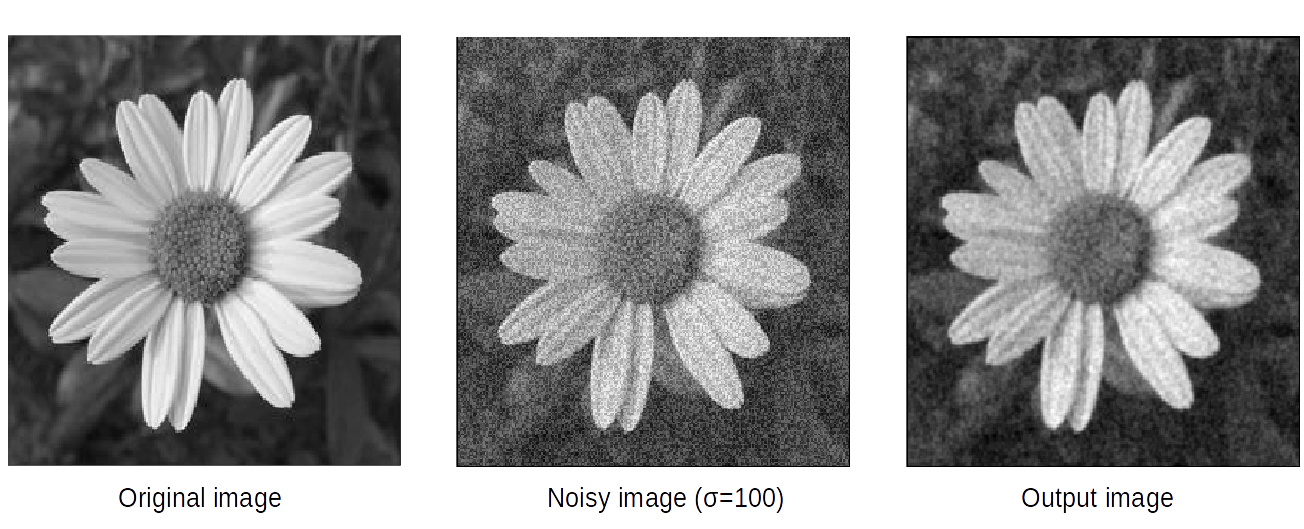
\includegraphics[width=\textwidth]{img/firstimpl.png} % TODO retake this picture maybe

We observe that the output picture is still quite noisy and blurry, we can certainly do better.

\subsection{Algorithm variations}


\subsubsection{Sampling method}
The sample required less than 1\% of the pixels of the image. To achieve this, we can use different approaches. The chosen method is decisive for the Nystr\"om method.
\begin{description}[align=left]
 \item [Random sampling (RS)] most common and simple sampling scheme, but no deterministic guarantee of the output quality. Can produce good results for images with poor resolution, but with a huge amount of data, random sampling is limited because it cannot reflect the structure of the data set \cite{zhan_improved_2017}.
 \item [K-means sampling (KS)] associate to each pixel a 5-D space (R, G, B, X, Y) and divide the pixels into K clusters (K centers). These clusters are a good sampling scheme for images with simple and uniform backgrounds \cite{kao_sampling_2012} \cite{zhang_improved_2008}.
 \item [Uniform spatially sampling] the uniformity of the sample gives good results for image sampling because of the spatial correlation of pixels. This method remains simple but effective \cite{glide_2014}.
 \item [Incremental sampling (INS)] is an adaptive sampling scheme, meaning that it select points according to the similarity, so that we can have an approximate optimal rank-k subspace of the original image \cite{zhan_improved_2017}.
 \item [Mean-shift segmentation-based sampling] this scheme performs good for complex backgrounds. The method consists in over-segmenting the image into \(n\) regions and only one pixel of each region will be sampled using the spatially closest pixel to the center of the region given a formula in \cite{kao_sampling_2012}.
\end{description}

\subsubsection{Affinity function}
The kernel function \(K_{ij}\) measures the similarity between the pixel \(y_i\) and \(y_j\).

\paragraph{Listing}

\begin{description}[align=left]
 \item [Spatial Gaussian Kernel] takes into account only the spatial distance between two pixels \cite{siam_slides_2016}.
 \item [Photometric Gaussian Kernel] considers the intensity and color similarity of the pixels \cite{siam_slides_2016}.
 \item [Bilateral Kernel] one of the most used kernel which smooths images by a nonlinear combination of the spatial and photometric gaussian kernels \cite{siam_slides_2016} \cite{glide_2014}.
 \item [Non-Local Means (NLM)] is similar to the bilateral kernel, a data-dependent filter, except that the photometric affinity is captured patch-wise \cite{glide_2014}.
 \item [Locally Adaptive Regression Kernel (LARK)] uses the geodesic distance based on estimated gradients \cite{milanfar_symmetrizing_2013} \cite{takeda_kernel_2007}.
\end{description}

\paragraph{Examples}

To illustrate the impact of the affinity function, here are some examples of the affinity matrix for certain pixels.
The more a pixel is colored in red, the more similar it is to the selected pixel, with respect to the chosen function.
A blue colored pixel is dissimilar to the considered pixel.

To generate these examples, we use an image of a house of dimension 200x300 pixels. Generating the affinity matrix takes approximately 160 seconds on an Intel i5 processor and the generation takes not much more than a 1 GB of memory. We use a spatially uniform sampling technique and select 1\% of the pixels. We show two affinity matrices for each techniques, the first one is on the grass in front of the house and the second on the roof.

\paragraph{Spatial Gaussian Kernel}
The formula of this kernel is
\[K(x_i, x_j) = exp(-||x_i - x_j||^2 / h_x^2).\]

Affinity matrices with \(h_x = 5\): \\
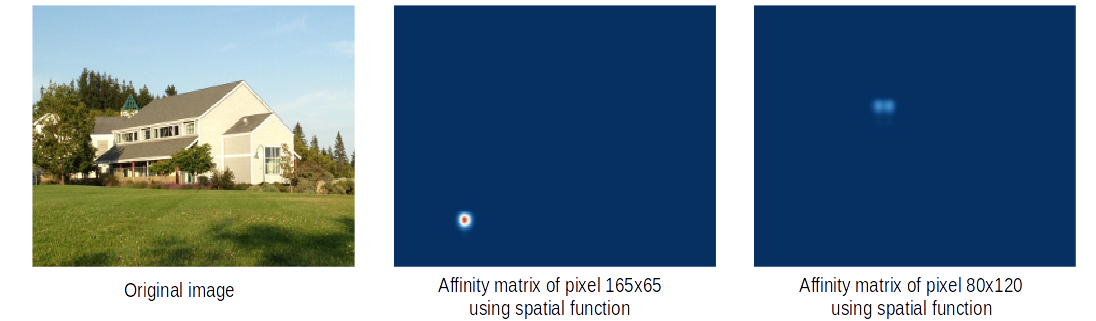
\includegraphics[width=\textwidth]{img/spatialAffinitySigma5.png}

Affinity matrices with \(h_x = 50\): \\
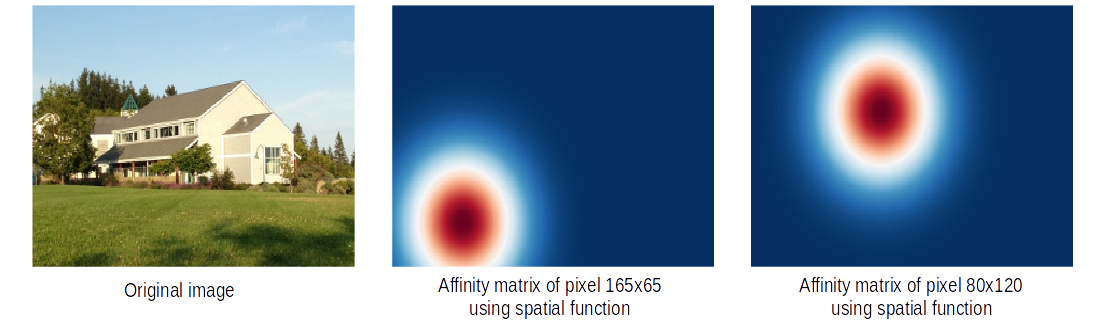
\includegraphics[width=\textwidth]{img/spatialAffinitySigma50.png}

As we can see, the parameter is influencing on the normalisation of the values and gaussian standard deviation.
The bigger is it, the more tolerant the spatial distance computation will be.

\paragraph{Spatial Gaussian Kernel}
The formula of this kernel is
\[K(z_i, z_j) = exp(-||z_i - z_j||^2 / h_z^2).\]

Affinity matrices with \(h_z = 5\): \\
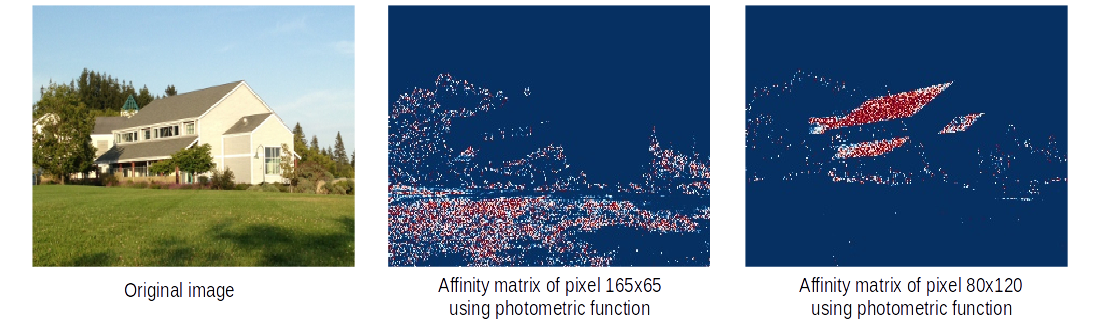
\includegraphics[width=\textwidth]{img/photometricAffinitySigma5.png}

Affinity matrices with \(h_z = 50\): \\
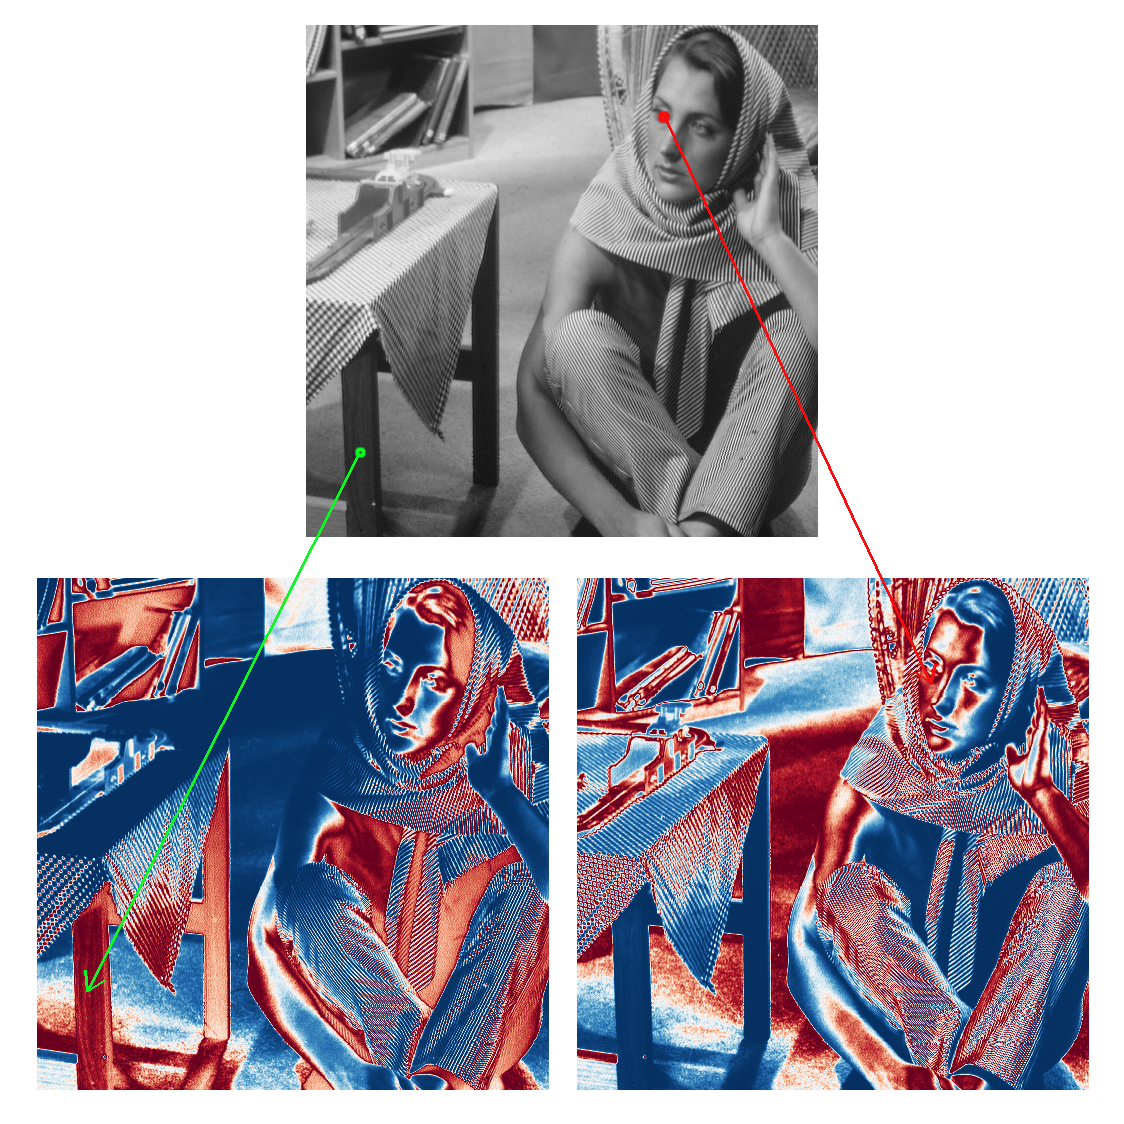
\includegraphics[width=\textwidth]{img/photometricAffinitySigma50.png}

Generally, the \(h\) parameters in both kernel functions here are smoothing parameters.
If \(h\) is small, it is more discriminating between the affinity of different pixels.

\paragraph{Bilateral Kernel}
Affinity matrices with \(h_x = 40\) and \(h_z = 30\): \\
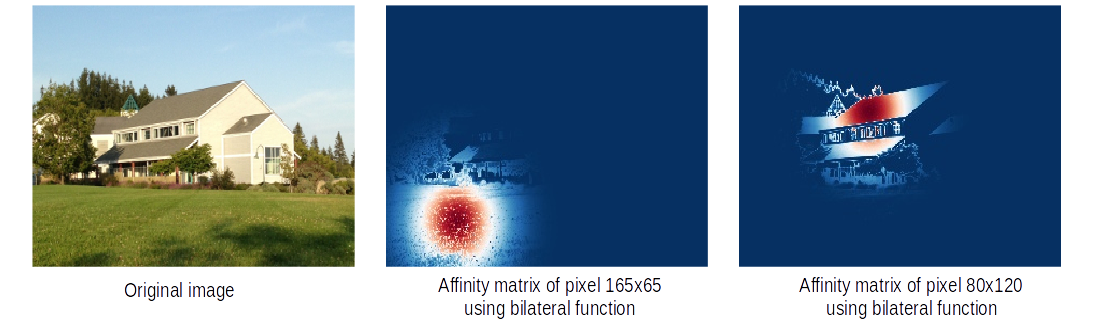
\includegraphics[width=\textwidth]{img/bilateralAffinitySpatial40Photo30.png}

Remember that each matrix here is only the affinity matrix of one pixel.
In a very heterogeneous image, the bilateral kernel will be useful to keep the spatial similarity, but with excluding very dissimilar neighbour pixels.

\subsubsection{Graph Laplacian}
Graph Laplacian has multiple possible definitions and each has its own properties.
A good summary can be found in \cite{siam_slides_2016}.
A Graph Laplacian can be symmetric which is important for eigen-decomposition of the matrix.
It can have a DC eigenvector, which means that the Laplacian has to give 0 if we apply it to a constant image. This is also useful to have.
And the spectral range, corresponding to the range of the eigenvalues, is important because we will use the filters derived from the Laplacian multiple times, and if the eigenvalues are not between 0 and 1, then the filters tend to be unstable.
With \(K\) being the affinity matrix, \(d_i = \sum_j K_{ij}\) and \(D = diag{d_i}^n_1\):

\begin{table}[!htbp]
 \centering
 \begin{tabular}{|c|c|c|c|c|}
  \hline
  Laplacian Name & Formula & Symmetric & DC eigenvector & Spectral Range \\
  \hline
  Un-normalised & \(D - K\) & Yes & Yes & [0, n] \\
  \hline
  Normalised & \(I - D^{-1/2}KD^{-1/2}\) & Yes & No & [0, 2] \\
  \hline
  Random Walk & \(I - D^{-1}K\) & No & Yes & [0, 1] \\
  \hline
  ``Sinkhorn" \cite{milanfar_symmetrizing_2013} & \(I - C^{-1/2}KC^{-1/2}\) & Yes & Yes & [0, 1] \\
  \hline
  Re-normalised & \(\alpha(D - K)\), \(\alpha = \bigO(n^{-1})\) & Yes & Yes & [0, 1] \\
  \hline
 \end{tabular}
\end{table}

Generally, it is a good practice to stick to one definition of the Laplacian.

\subsection{Adaptive Sharpening}

Sharpening is usually using a highpass filter and therefore leads to amplifying high frequency noise components even more.
We will have an effect of oversharpening.

\(\beta \) controls the amount of sharpening of the image.

\clearpage
\printbibliography

\end{document}
